\documentclass[class=scrartcl, crop=false]{standalone}


\graphicspath{ {./lectures/images/}{./images/} }

\title{Comp 598 Notes}
\date{05-05}


\begin{document}

\section{05-05}

\subsection{Quantifiers}

Can think of $\exists$ as Eloise and $\forall$ as Abeland. Think of statements
as a game between these two. The statement is true if Eloise has a winning
strategy, and false otherwise (i.e. Abeland has a winning strategy).

\subsection{Design a machine that accepts string ending in "aa".}

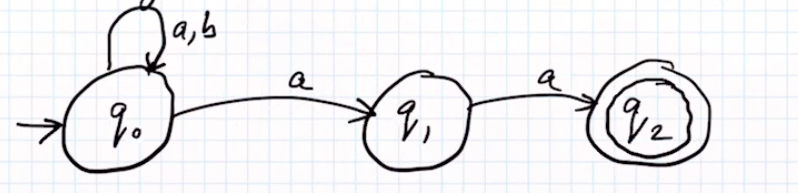
\includegraphics[width=\textwidth]{nondeterministic_finite_automaton}
\subsection{NFA vs DFA}
\begin{enumerate}
  \ii There can be multiple next states or no next state. NFA's can make
  choices. There are multiple computation paths corresponding to different
  choices. A word is \ul{accepted} if there exists a path leading to an accept
  state.

\end{enumerate} 
If a machine jams, that is equivalent to rejection. Therefore only sequences
that end with "aa" can end up at the accept state.

\begin{theorem}
  The language accepted by any NFA is a regular language. i.e. could also have
  been accepted by a DFA.
\end{theorem}
\begin{remark}
  There is an \ul{algorithm} for converting an NFA into an \ul{equivalent} DFA.
  So you can go crazy with an NFA and know that it is still a regular language.
\end{remark}

\begin{note}
  Another extension: NFA + $\epsilon$ This machine can make jumps wihtout
  reading any input.
  \begin{gather*}
    DFA \equiv NFA \equiv NFA + \epsilon \equiv \text{Regular Languages}
  \end{gather*}
\end{note}


\begin{example}[Decimal Numbers]
  $\pm$ in front, optional. Two sequences of digits with one or the other (but not both) potentially empty. The goal is to add numbers. \\
  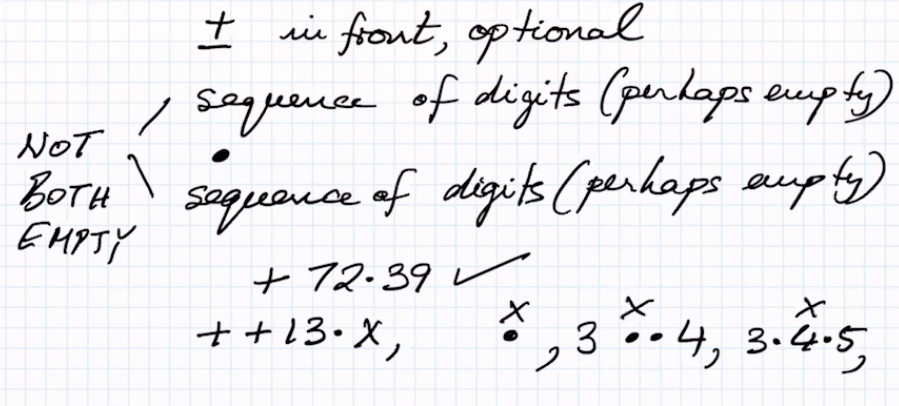
\includegraphics[width=\textwidth]{decimal_example.png}

  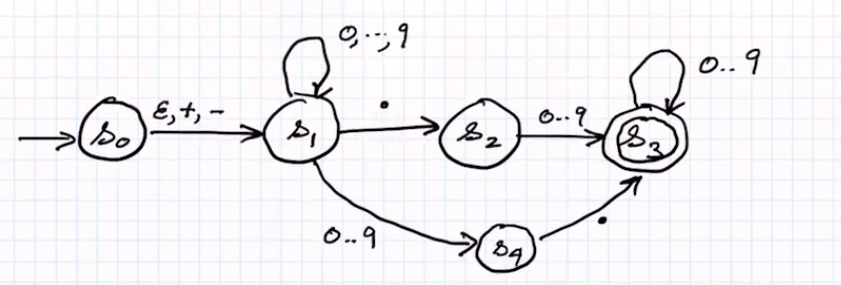
\includegraphics[width=\textwidth]{decimal_example_dfa.png}

  \begin{enumerate}
    \ii Exactly plus, or exactly minus, or nothing. Otherwise the machine will
    jam. \ii $\epsilon$ is not just "hey I can jump to anywhere at any time"; it
    is part of the design of the machine. \ii There should be at least one thing
    after the decimal point. \ii No transition for another dot or plus or minus
    so any of those would cause the input to get rejected. \ii Allow for the
    possibility of ending with decimal point. \ii Need to two path to acceptance
    to distinguish between either before the decimal or after the decimal being
    empty, but not both.
  \end{enumerate}
  This thing is doing a lot of guessing.
\end{example}

\begin{note}
  In order to accept the language, it most both accept the right things and
  reject the wrong things. Cannot just accept everything.
\end{note}

\begin{definition}[Formal definition of NFA]
  An NFA is a 4-tuple:
  \begin{enumerate}
    \ii $Q$: a finite set of states \ii $Q_0 \subseteq Q$ : a (finite) set of
    \ul{start} states \ii $F \subseteq Q$ : a (finite) set of \ul{accept} states
    \ii
    $\Delta$ :  $ Q \times \Sigma \to 2^Q$. \\
    Or with $\epsilon$. $\Delta : Q \times (\Sigma \cup \{\epsilon\}) \to 2^Q$
    \begin{align*} % review
      &\Delta^* : Q \times \Sigma^* \to 2^Q \\
      &\Delta^*(q, \epsilon) = \{q\} \\
      &\Delta^* (q, w \cdot a) = \cup_{q' \in \Delta^*(q, w)}\Delta(q', a)
    \end{align*} 
    \ii The accept state
    \begin{gather*}
      L(N) = \{w \in \Sigma^* \ | \ \exists q \in Q_0, \Delta^*(q, w) \cap F \neq
      \varnothing\}
    \end{gather*}
  \end{enumerate}
  
\end{definition}

\begin{theorem}
  Given an NFA $N = (Q, Q_0, F, \Delta)$ there is a DFA $M = (S, s_0, F', \delta)$
  such that $L(N) = L(M)$.
  \begin{proof}
    Keep track of all the places where the m/c (machine) could be.
    \begin{gather*}
      S = 2^q \\
      s_0 = Q_0 \\
      F' = \{S \subseteq Q \ | \ S \cap F \neq \varnothing\} \\
    \end{gather*}
    Take the union of all the places where it could go. % review
    \begin{gather*}
      \delta(s, a) = \cup_{q \in s} \Delta(q, a)
    \end{gather*}
    It is easy to see that this works (favorite line of math professors) as
    advertised.
  \end{proof}
  \begin{remark}
    It is possible to have an exponential blow up in the number of states.
  \end{remark}
\end{theorem}
\begin{note}
  $S = 2^Q$ refers to the set of all subsets of Q (power set). The power set of $S$ can be identified with the set of all functions from $S$ to a given set of two elements $2^S$. \\\\
  This can be understood where you represent each of the elements in the set as
  a digit in a binary number. Then, in order to find all possible sets, you
  would find all possible binary numbers with $|S|$ digits, which gives
  $2^{|S|}$.
\end{note}

For $NFA + \epsilon$ we define $\epsilon$-closure of a set to be the places one
can get to with an $\epsilon$-move. % review

\begin{example}
  Let $L$ be a regular language. Let $\frac{1}{2}L = \{w \in \Sigma^* \ | \
  \exists x \in \Sigma^*, wx \in L \ \wedge \ |w| = |x|\}$.
  \\\\
  Look at left half of word and guess that there is something you can tack on to
  the right such that the entire word is something the original machine would
  recognize.
  \\\\
  Assume DFA $(S, s_0, F, \delta)$ recognizes $L$. We will construct an NFA for
  $\frac{1}{2}L$.
  \begin{gather*}
    Q = S \times S \times 2^S
  \end{gather*}
  First index for . Second index for guessing where $DFA$ will be when $w$ ends.
  Third index is to try and track $x$ the second half of the word.
  \begin{gather*}
    Q_0 = \{(s_0, s, \{s\})\} \\
    F' = \{(s, s, X) \ | \ X \cap F \neq \varnothing\} \\
    \Delta((s, \ol{s}, X), a) = \{(s', \ol{s}, X') \ | \ \delta(s, a) = s'\}
  \end{gather*}
  where $X'$ is the set of states DFA can reach from $x$ reading any
  symbol. % review
\end{example}

Closure properties of regular languages.
\begin{enumerate}
  \ii $L_1 \cap L_2$ is regular. Define a machine for $L_1$ and $L_2$. You
  create a state space with the cartesian product of states for $L_1$ and $L_2$.
  Then you go through in parallel and if it's in the accept state of both then
  it's accepted. \ii
  $L_1 \cup L_2$ is regular. \\
  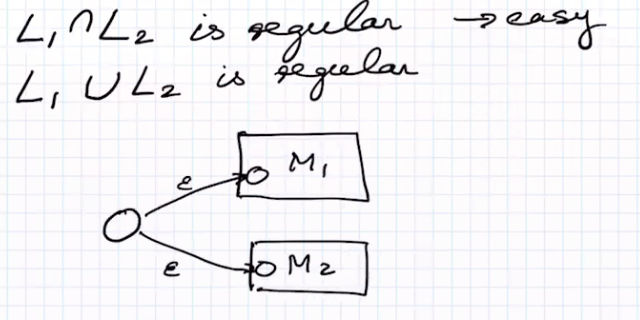
\includegraphics[width=\textwidth]{closure_union} \ii
  Concatenate language. $L_1 \cdot L_2 = \{x \cdot y \ | \ x \in L_1, y \in L_2\}$. \\
  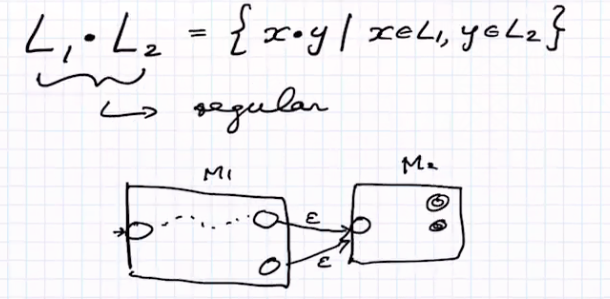
\includegraphics[width=\textwidth]{closure_concatenate} \ii If $L$ is a
  language, $L^*$ is a new language where
  \begin{gather*}
    L^* = \{w_1 \cdots w_k \ | \ w_i \in L\} \cup \{\epsilon\}
  \end{gather*}
  Basically take as many words as you like and glue them all together. Called the kleene (clay-knee) star operator. If $L \ \text{is regular} \Rightarrow L^* \ \text{is regular}$ but not the other way around. \\
  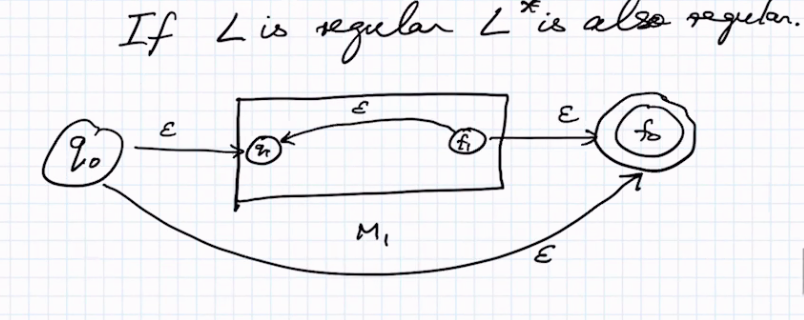
\includegraphics[width=\textwidth]{closure_star} \ii Shuffle.
  \begin{gather*}
    L_1 // L_2 = \{x_1y_1x_2y_2 \cdots x_ky_k \ | \ x_1x_2 \cdots x_k \in L_1, \
    y_1 y_2 \cdots y_k \in L_2\}
  \end{gather*}
\end{enumerate}

\subsection{Regular Languages as an algebra}

\begin{definition}[Regular expressions]
  Notation for describing regular languages in a machine independent fashion.
  \begin{enumerate}
    \ii If $R_1, R_2$ are regular expressions, then $R_1 + R_2, \ R_1 \cdots
    R_2$ are regular expressions.
    \\\\
    If $R$ is a regular expression, $R^*$ is a regular expression.
    \\\\
    A regular expression denotes a language.
    \begin{gather*}
      \llbracket \varnothing \rrbracket = \varnothing, \\
      \llbracket \epsilon \rrbracket = \{\epsilon\}, \\
      \llbracket R_1 \cdot R_2 \rrbracket = \llbracket R_1 \rrbracket \cdot \llbracket R_2 \rrbracket, \\
      \llbracket R^* \rrbracket = (\llbracket R \rrbracket)^* / \llbracket
      \ol{R} \rrbracket = \ol{(\llbracket R \rrbracket)}
    \end{gather*}
    \begin{example}
      $(aa + b)^* = \{aa, \epsilon, b, aab, bbaab, \cdots \}$
    \end{example}
  \end{enumerate}
  \begin{theorem}[Kleene Theorem]
    A language is regular iff it can be described by a regular expression.
    \begin{proof}
      Easy to see that reg exp implies regular. We already showed relevant
      closure properties. Reverse direction later if even.
    \end{proof}
  \end{theorem}
  \begin{note}
    "+" is notation for "or".
  \end{note}
  We have a set of equational axioms for reasoning about equality of regular
  expressions. Reg set of regular expressions (without -). \\ % review
  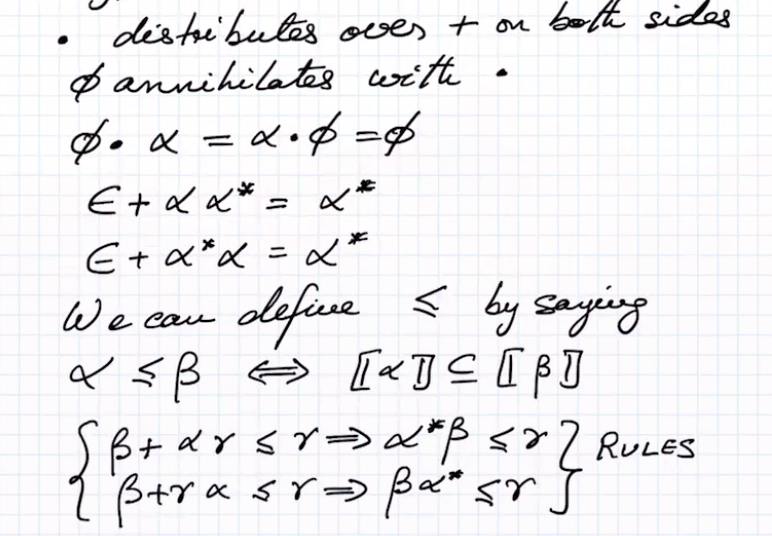
\includegraphics[width=\textwidth]{reg_rules}
  \begin{theorem}
    These rules are complete. i.e. every valid equation can be derived from
    these rules.
  \end{theorem}
  \begin{remark}
    In order to do anything algorithmic, use DFA. \\
    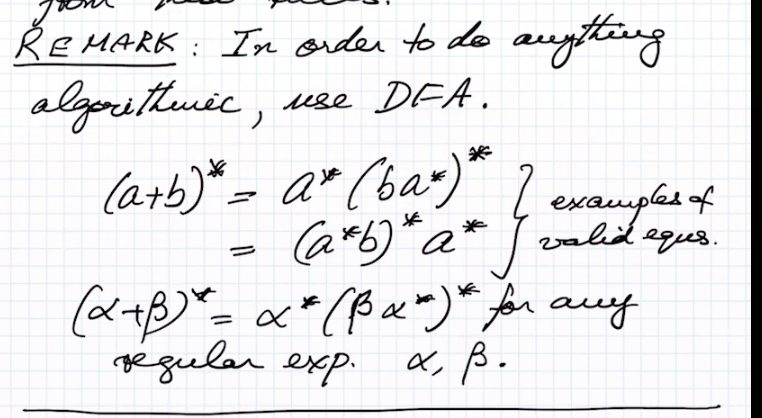
\includegraphics[width=\textwidth]{more_rules}
  \end{remark}
\end{definition}

\subsection{From DFA to reg exp}
Enumerate the states of a DFA $1, 2, \dots, k$. For every pair of states $i, j$
we define $R_{ij}^n$ as a regular expression describing all strings that take the
DFA from $i$ to $j$ only traversing states $1, \dots, n$ along the way.
\begin{example}
  $R_{ij}^0$ would represent only direct jumps from $i$ to $j$. Either the empty
  word, or a single symbol.
  \\\\
  We can compute $R_{ij}^{n + 1}$ from $R_{ij}^n$. Then you can build the DFA by
  union all regular expressions describing jumps from start to accept states.
  \\
  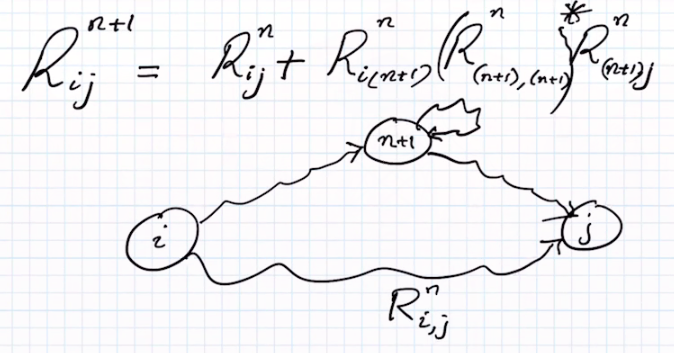
\includegraphics[width=\textwidth]{calculating_up}
\end{example}

\end{document}
